\chapter{Problem Statement and Background}

\section{Introduction}
This chapter introduce the topic of the thesis. It defines the problem statement and also give a brief background about it.
\section{Background}
Administrative data systems currently rely on the Central Personal Register Id (CPR Nr.) to link customer data with a real world identity. This means that almost all data managed by the institutions must be classified as personal identifiable information and therefore managed according to strict confidentiality requirements as well as integrity and availability requirements. The purpose of this thesis project is to examine ways to decouple transaction data from the underlying identities, so that the data used in the institution's day to day operations are decoupled from the underlying customer identity. This limits the confidentiality requirements for the data and the vulnerability to insider threats, such as the recent leak of celebrity data from NETS to the magazine "Se \& Hør". It must, however, be possible to link customer data to real world identities when reporting financial data to the Tax authorities or in connection with suspicions about criminal activity, e.g. fraud, insider trading, whitewashing, etc. Austria is already considering similar approaches in the public health care system, where the health records of the citizens are saved under pseudonyms, which are mapped one-to-one to the single citizen.
\section{Definitions}
Here we will give some of the definitions used in the system
\subsection{Privacy}
\subsection{Anonymity}
\subsection{Pseudonym}
\subsection{User}
\subsection{Bank}
\subsection{Third party}
\subsection{Service}
\subsection{Unlinkability}
\subsection{Revocation}
\subsection{Partial Information Disclosure}
\subsection{Conditional Anonymity Removal}
\subsection{Legal Requirement}
\section{Case Study}
Nykredit is a major financial institution in Denmark providing different services, such as mortgages, retail banking, investment banking etc. They also are part of a big group of companies, which includes other financial institutions providing similar services. These financial institutions basically provide Nykredit services as their own services to the customers.
Nykredit has mainly 2 types of customers:
\begin{itemize}
\item Private Customers
\item Corporate Customers
\end{itemize}
\begin{figure}[h]
	\centering
	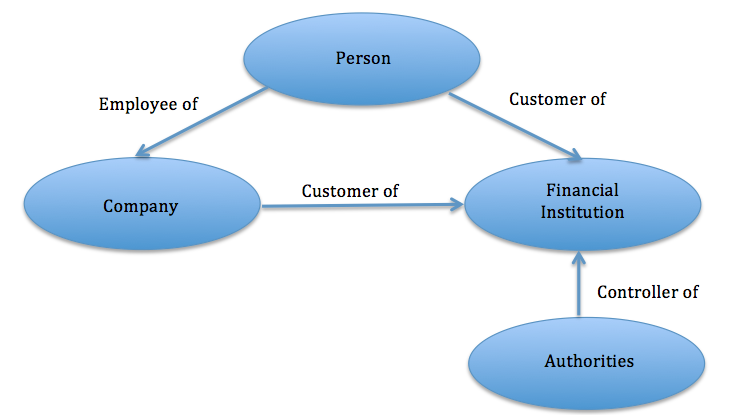
\includegraphics[width=\textwidth]{figures/Customers}
	\caption{Identities in the system}
	\label{fig:Customers}
\end{figure}
\subsection{Private Customers}
Private customers are the individual customers who access Nykredit services on their own. Usually there is a single person accessing the services of the bank. These customers are usually people who get a personal bank account with Nykredit.
\subsection{Corporate Customers}
Corporate customers are either companies who are customers of Nykredit or other financial institutions which provide Nykredit services to their own private customers. Usually there are many people who access Nykredit services on behalf of the corporate customer.
\section{Problem}
We consider the case of a person, who may either be a private customer of Nykredit, or an employee of a company who is corporate customer of Nykredit. In this case, the person may also be responsible for managing the accounts of his employer with Nykredit.
\\
\\Nykredit wants to setup an identity management system so that there is no need for the individual to disclose his personal identity to Nykredit to access the account on behalf of the company.
\\Nykredit, however, also have to comply with relevant legislation (KYC, AML, “Hvidvaskningsloven”),  e.g. in case the authorities (Tax, Police, etc.) find some suspicious transactions. Nykredit needs to provide the identity of the person responsible for these transactions.
This means that it is required that Nykredit, in case of a legal request, is able to identify the individual employee from the institution, who is accessing the account on the corporate customer’s behalf.
\\
\\So the main goal of the system is:
\begin{itemize}
	\item Nykredit should not learn identity of the individual person accessing the services on behalf of corporate customer.
	\item For complying with legislation Nykredit should be able to map real identity of the individual person with the transaction in case its required by the law.
\end{itemize}
The project will perform an initial analysis of a single business process from administrative data management, with respect to identifying the need to bind authenticated identities to actions at the different steps of the process; this analysis will be presented to stakeholders from the specific administrative domain. Based on the initial analysis of the selected business process, the project will develop a full identity model for the chosen business process with anonymisation and pseudonymisation of actors whenever possible. The feasibility of the proposed model will be evaluated through a prototype that implements the model using standard components from identity management infrastructures whenever possible.
\section{Summary}
Companies do not want to disclose the personal identity of their employees to Nykredit, but they still need the ability to access all services online. Managing all identities, while maintaining privacy, is not easy and provides different challenges. We have to design a system, which fulfill the entire privacy requirement and still enables Nykredit to provide its services to its customers and meet the regulatory requirements of the authorities without any problem.
 